\documentclass{article}

\usepackage[tmargin=0.5in,bmargin=0.25in]{geometry}
\usepackage{amsmath, amssymb, amsthm}
\usepackage{enumitem}
\usepackage{graphicx}
\graphicspath{{./}}

\title{\vspace{-4ex}Math 341 Homework 6}
\author{Isaac Boaz}

\renewcommand{\arraystretch}{1.2}

\begin{document}

\maketitle

\section*{Problem 2}

Let \(X\) be a random variable representing the number of shooting stars per hour. Assume \(X\) is Poisson distributed with \(E[x] = \lambda\) (i.e: \(X \sim Poisson(\lambda)\)).

\begin{enumerate}[label=\alph*)]
    \item Instead of a 1-hour interval, consider an interval of \(t\) hours where \(t > 0\). If \(Y\) denotes the number of stars in \(t\) hours, what is its distribution and parameter value?
          \begin{align*}
              Y \sim Poisson(t\lambda)
          \end{align*}
    \item Calculate the probability that no shooting stars are observed in \(t\) hours (i.e: \(P(Y = 0)\)).
          \begin{align*}
              P(Y = y) = \frac{e^{-t\lambda} \cdot (t\lambda)^y}{y!}
          \end{align*}
          \begin{align*}
              P(Y = 0) & = \frac{e^{-t\lambda} \cdot (t\lambda)^0}{0!} \\
                       & = \frac{e^{-t\lambda}}{1}                     \\
                       & = e^{-t\lambda}                               \\
          \end{align*}
    \item Suppose we measure the time (\(T\)) until the first shooting star. Explain why the event \(A = \{T > t\}\) is equivalent to the event \(B = \{Y = 0\}\)
          \begin{description}
              \item Event \(B\) represents the event that no shooting stars are observed in \(t\) hours.
              \item Event \(A\) represents the event that the first shooting star is observed after \(t\) hours.
              \item Since event \(A\) is defined as \(T > t\), we know that at least \(t\) hours have passed before the first shooting star is observed.
          \end{description}
    \item Using (c), compute the cdf of \(T\). Then, state the distribution of \(T\) and its parameter value.
          \begin{align*}
              A = B    & \implies P(A) = P(B) \\
              P(T > t) & =  P(Y = 0)          \\
                       & = e^{-t\lambda}      \\
          \end{align*}
          \begin{align*}
              \text{CDF of T: } F(t) =  P(T \leq t) \\
              = 1 - e^{-t\lambda}
          \end{align*}
          \(T\) represents an exponential distribution with parameter \(\lambda\).
\end{enumerate}

\pagebreak

\section*{Problem 7}
\(X\) is a random variable for the \% of degree holders where \(\mu = 31.22,\ \sigma = 5.3\).

\begin{enumerate}[label=\alph*)]
    \item Using a normal distribution, compute the proportion of countries where \(\geq 40\%\) have a degree.
          \begin{align*}
              P           & (X \geq 40)          \\
              X      \sim\ & N(31.22, 5.3^2) \\
              \mathcal{Z} =\ & (X - \mu)/\sigma
          \end{align*}
          \begin{align*}
              P(X \geq 40)  & = P(\frac{x\mu}{\sigma} \geq \frac{40-\mu}{\sigma}) \\
              P(\mathcal{Z} & \geq\frac{40-31.22}{5.3})                           \\
                            & = 1 - P(\mathcal{Z} \leq 1.657)                     \\
                            & = 1 - \text{pnorm(1.657)}                           \\
                            & = 1 - 0.9512403 = 0.0487597
          \end{align*}
    \item Let \(Y\) denote per capita income represented by \(Y = 45000 + 1.7X\).
          \begin{align*}
              Y = aX+b, \mu = au+b, \sigma = a^2\sigma^2
          \end{align*}
          We know that \(Y = aX + b\) can be represented as a Normal Distribution such that:
          \begin{align*}
              Y \sim N(a\mu + b, a^2\sigma^2)
          \end{align*}
          Plugging in the values for \(a, b, \mu, \sigma\):
          \begin{align*}
              \mu_y = 1.7\cdot 31.22 + 45000 = 45053.074 \\
              \sigma_y^2 = 1.7^2\cdot 5.3^2 = 81.1801
          \end{align*}
          As such, \(Y\) is normally distributed with \(\mu_y = 45053.074\) and \(\sigma_y^2 = 81.1801\).
          %   The distribution of \(Y\) is normal with mean \(\mu = 45000 + 1.7\cdot 31.22 = 45000 + 53.474 = 45053.474\) and standard deviation \(\sigma = 1.7\cdot 5.3 = 8.91\).
    \item Calculate \(c\) such that \(P(|Y-45053.07| < c) = 0.758\)
          \begin{align*}
              P(-c <                                 & Y-45053.07 < c)              = 0.758                                                                   \\
                                                     & = P(-c + 45053.07 < Y < c + 45053.07)                                                                  \\
                                                     & = P(\frac{-c+45053.07-\mu_y}{\sigma_y} < \frac{Y-\mu_y}{\sigma_y} < \frac{c+45053.07-\mu_y}{\sigma_y}) \\
                                                     & = P(\frac{-c}{\sigma_y} \leq \mathcal{Z} < \frac{c}{\sigma_y})                                         \\
                                                     & = 1 - 2P(\mathcal{Z} \leq \frac{-c}{\sigma_y})                                                         \\
              P(\mathcal{Z}<                         & \frac{-c}{\sigma_y})      = \frac{1-0.758}{2}                                                          \\
                                                     & =                                  0.121                                                               \\
              _{\mathcal{Z}}                         & = \frac{c}{\sigma_y}                                                                                   \\
              P(\mathcal{Z\leq_{\mathcal{Z}}})       & = 0.121                                                                                                \\
              _{\mathcal{Z}} & = \text{invNorm(0.121)} = -1.1700                                                                                              \\
              c                                      & = -1.17 \cdot \sigma_y                                                                                 \\
              c                                      & = -1.17 \cdot \sqrt{81.1801} = -10.54
          \end{align*}
    \item For any \(N\) with \(\mu \text{ and } \sigma^2,\ Q_1 - 1.5IQR = \mu - 2.68 \sigma\) and \(Q_3 + 1.5IQR = \mu + 2.68 \sigma\).
          \begin{align*}
              P(\mu - 2.68 & \sigma \leq X \leq \mu + 2.68 \sigma) \\
              & = P(-2.68 \leq \frac{X-\mu}{\sigma} \leq 2.68)     \\
              & = P(-2.68 \leq \mathcal{Z} \leq 2.68)               \\
              & = P(\mathcal{Z} \leq 2.68) - P(\mathcal{Z} \leq -2.68) \\ 
              & = 0.99632 - 0.00368          \\
              & = 0.99264
          \end{align*}
\end{enumerate}

\pagebreak

\section*{Problem 8}
The following data represents the annual total releases of TRI-covered chemicals to the environment:
\begin{align*}
     & \{33374, 32774, 24280, 26575, 26899, 13361, 13433, 43466, 13760, 10637\}               \\
     & \ \rightarrow \{ 10637, 13361, 13433, 13760, 24280, 26575, 26899, 32774,33374, 43466\}
\end{align*}

\begin{enumerate}[label=\alph*)]
    \item Compute the sample mean \((\overline{x})\) and sample standard deviation \(s\).
          \begin{align*}
              \overline{x} =                   & \sum_{n=1}^{k}     {\frac{x_k}{k}}                                         \\
                                               & = \frac{33374 + \dots + 10637}{10}                                         \\
              \overline{x}                     & \approx 23856                                                              \\
              s^2                            = & \frac{\sum_{i=1}^{n}(x_i-\overline{x})^2}{n-1}                             \\
              s^2                              & = \frac{(33374 - \overline{x})^2 + \dots + (10637 - \overline{x})^2}{10-1} \\
              s                                & \approx 10888.5
          \end{align*}
    \item 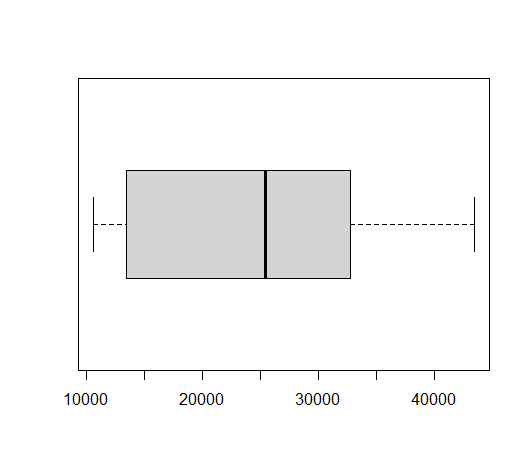
\includegraphics[scale=0.5]{boxplot.png}
    \item Does the data appear to be symmetric and/or skewed?
          \begin{enumerate}[label=(\roman*)]
              \item Symmetric
                    \begin{description}
                        \item Since the sample size is small, it would be very possible for more data to rebalance the Q1 and Q3 values. Additionally, the median line is visually close to the center.
                    \end{description}
              \item Skewed
                    \begin{description}
                        \item The data appears to be skewed to the left going off of the Q1 and Q3 offsets.
                    \end{description}
          \end{enumerate}
\end{enumerate}

\end{document}